\documentclass{article}
\usepackage[letterpaper,top=2cm,bottom=2cm,left=3cm,
            right=3cm,marginparwidth=1.75cm]{geometry}
\usepackage{graphicx}
\begin{document}
\begin{minipage}{0.9\textwidth}
    \centering
    \Large
    \textbf{ECE4144 – Communication Hands On Assignment}
\end{minipage}\\[1em]
The objective of this hands-on assignment is to implement a simple communication program based on USART built on the board. The processor has only one USART that is available to us, which is UART1 (instead of what written in the document). But according to the document and the datasheet, I have implemented the following code to fulfill requirements:
\begin{verbatim}
        /* UCSR0A is set as default. 
          Normal transmission speed, 
          disable the multi-processor communication mode */
        UCSR0A = 0x00;            // Reset the UCSR0A

        UCSR0B = 0x00;            // Reset the UCSR0B
        UCSR0B |= (1 << RXCIE1) | // Enable RX Complete Interrupt
                  (1 << RXEN1)  | // Enable Receiver
                  (1 << TXEN1);   // Enable Transmitter

        UCSR0C = 0x00;            // Reset the UCSR0C
        UCSR0C |= (1 << UCSZ11) | // Set Character Size to 8-bit
                  (1 << UCSZ10);
                  
        UBRR0 = 51;               // UBRR0 = (fosc / (16 * Baud Rate)) - 1
                                  //       = (8MHz / (16 * 9600)) - 1 = 51.08
\end{verbatim}
After following the requirements in question 2 and question 3, we can have the following code:
\begin{verbatim}
        #include <Arduino.h>

        char receivedByte = 0;
        
        void USART_Init() {
          /* UCSR0A is set as default. 
            Normal transmission speed, 
            disable the multi-processor communication mode */
          UCSR0A = 0x00;            // Reset the UCSR0A
        
          UCSR0B = 0x00;            // Reset the UCSR0B
          UCSR0B |= (1 << RXCIE1) | // Enable RX Complete Interrupt
                    (1 << RXEN1)  | // Enable Receiver
                    (1 << TXEN1);   // Enable Transmitter
        
          UCSR0C = 0x00;            // Reset the UCSR0C
          UCSR0C |= (1 << UCSZ11) | // Set Character Size to 8-bit
                    (1 << UCSZ10);
                    
          UBRR0 = 51;               // UBRR0 = (fosc / (16 * Baud Rate)) - 1
                                    //       = (8MHz / (16 * 9600)) - 1 = 51.08
        }
        
        ISR(USART0_RX_vect) {
          receivedByte = UDR0;      // Read the received byte
          
        }
        
        void TransmitString(const char* str, uint8_t length) {
          // Transmit byte by byte
          for (uint8_t i = 0; i < length; i++) {
            while (!(UCSR0A & (1 << UDRE0))) {
              // Wait for the transmit buffer to be empty
            }
            UDR1 = str[i]; // Transmit the byte
          }
        }
        
        char GetNextReceivedByte(){
          char byte;
          cli();               // Disable global interrupts
          byte = receivedByte; // Read the received byte
          receivedByte = 0;    // Clear the received byte after reading
          sei();               // Enable global interrupts
          return byte;
        }
        
        void setup() {
          USART_Init(); // Initialize USART0
          sei();        // Enable global interrupts
        }
        
        void loop() {
          char currentByte = GetNextReceivedByte();
          // Check if a byte is received
          if (currentByte != 0) {
            switch (currentByte) {
              case '1':
                TransmitString("One\n", 4);
                break;
              case '2':
                TransmitString("Two\n", 4);
                break;
              default:
                TransmitString("Default\n", 8);
                break;
            }
          }
        }  
\end{verbatim}
After uploaded the program to the board, I connected the board to the FTDI programmer like in the figure below:
\begin{figure}[h]
    \centering
    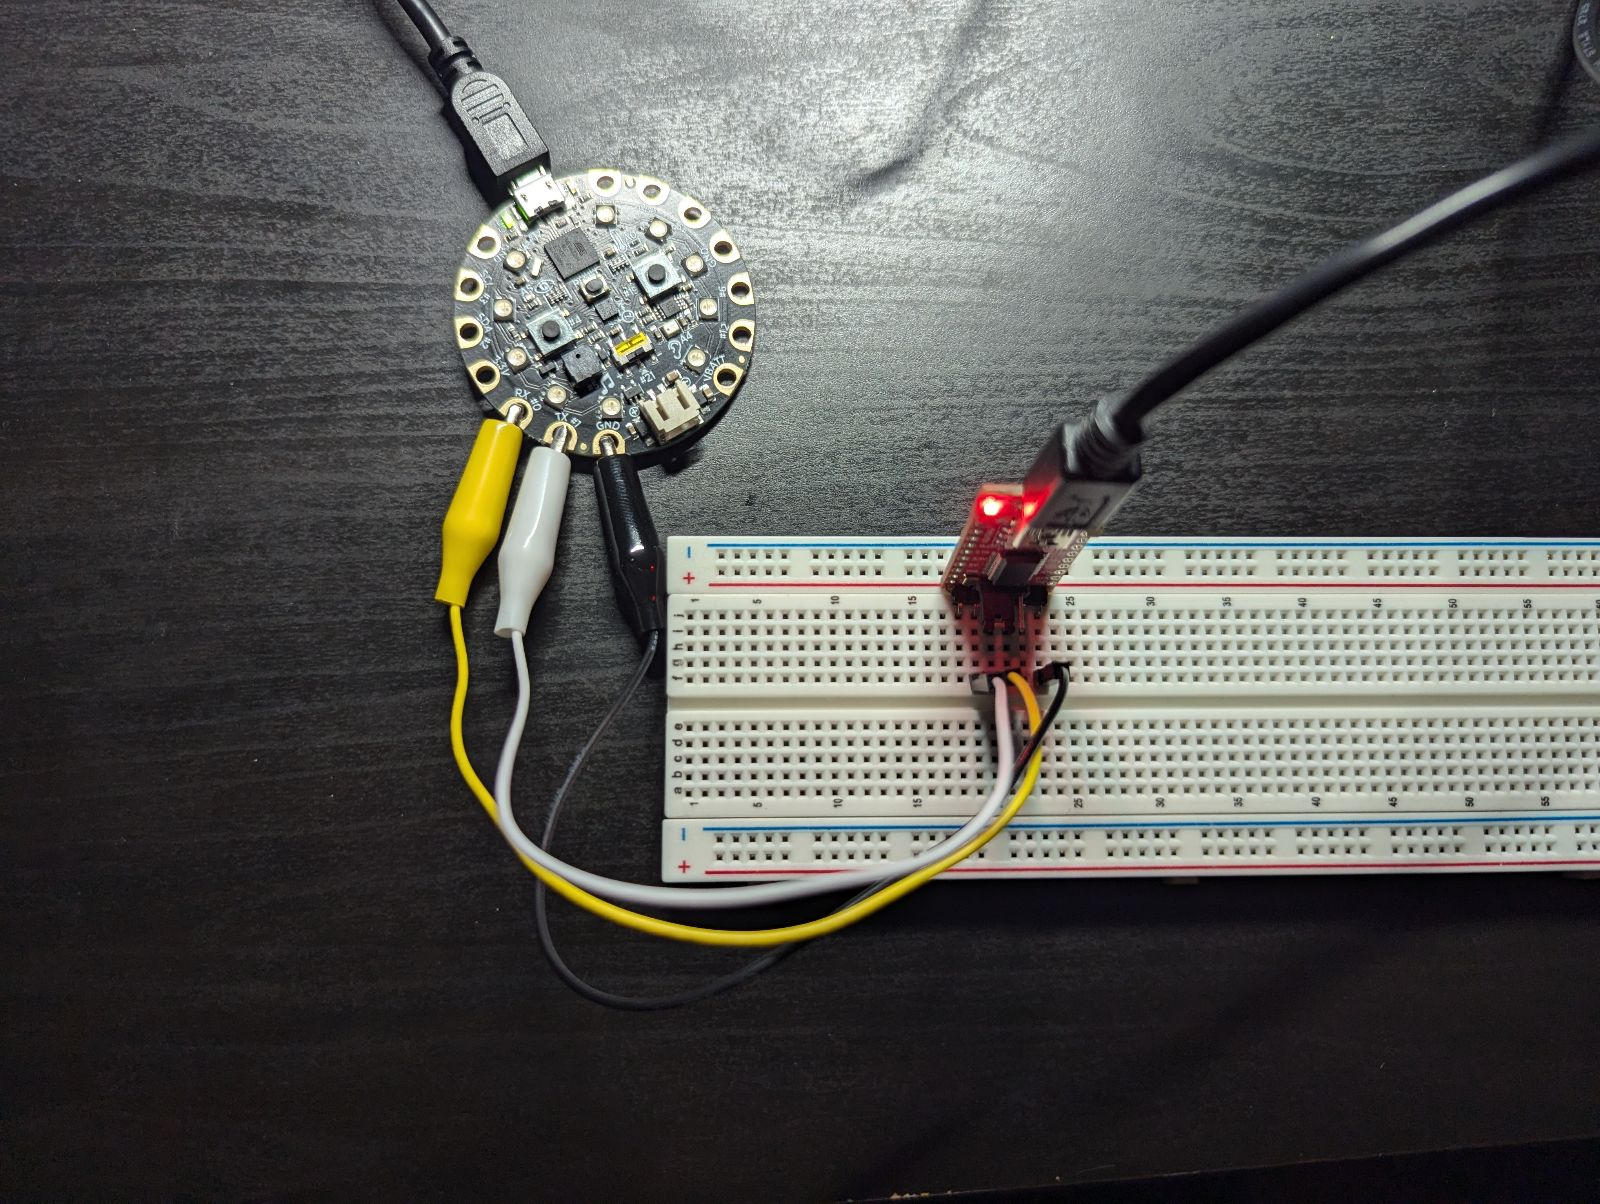
\includegraphics[width=0.5\textwidth]{pic1.png}
    \caption{Connection between the board and the FTDI programmer}
\end{figure}\\
Since we can only access the USART1, so for the part of implementing and testing, I switched to USART1. Then, I opened the serial monitor in the Tera Term and typed along the commands. Then, I received the outputs like in the figure below:
\begin{figure}[h]
    \centering
    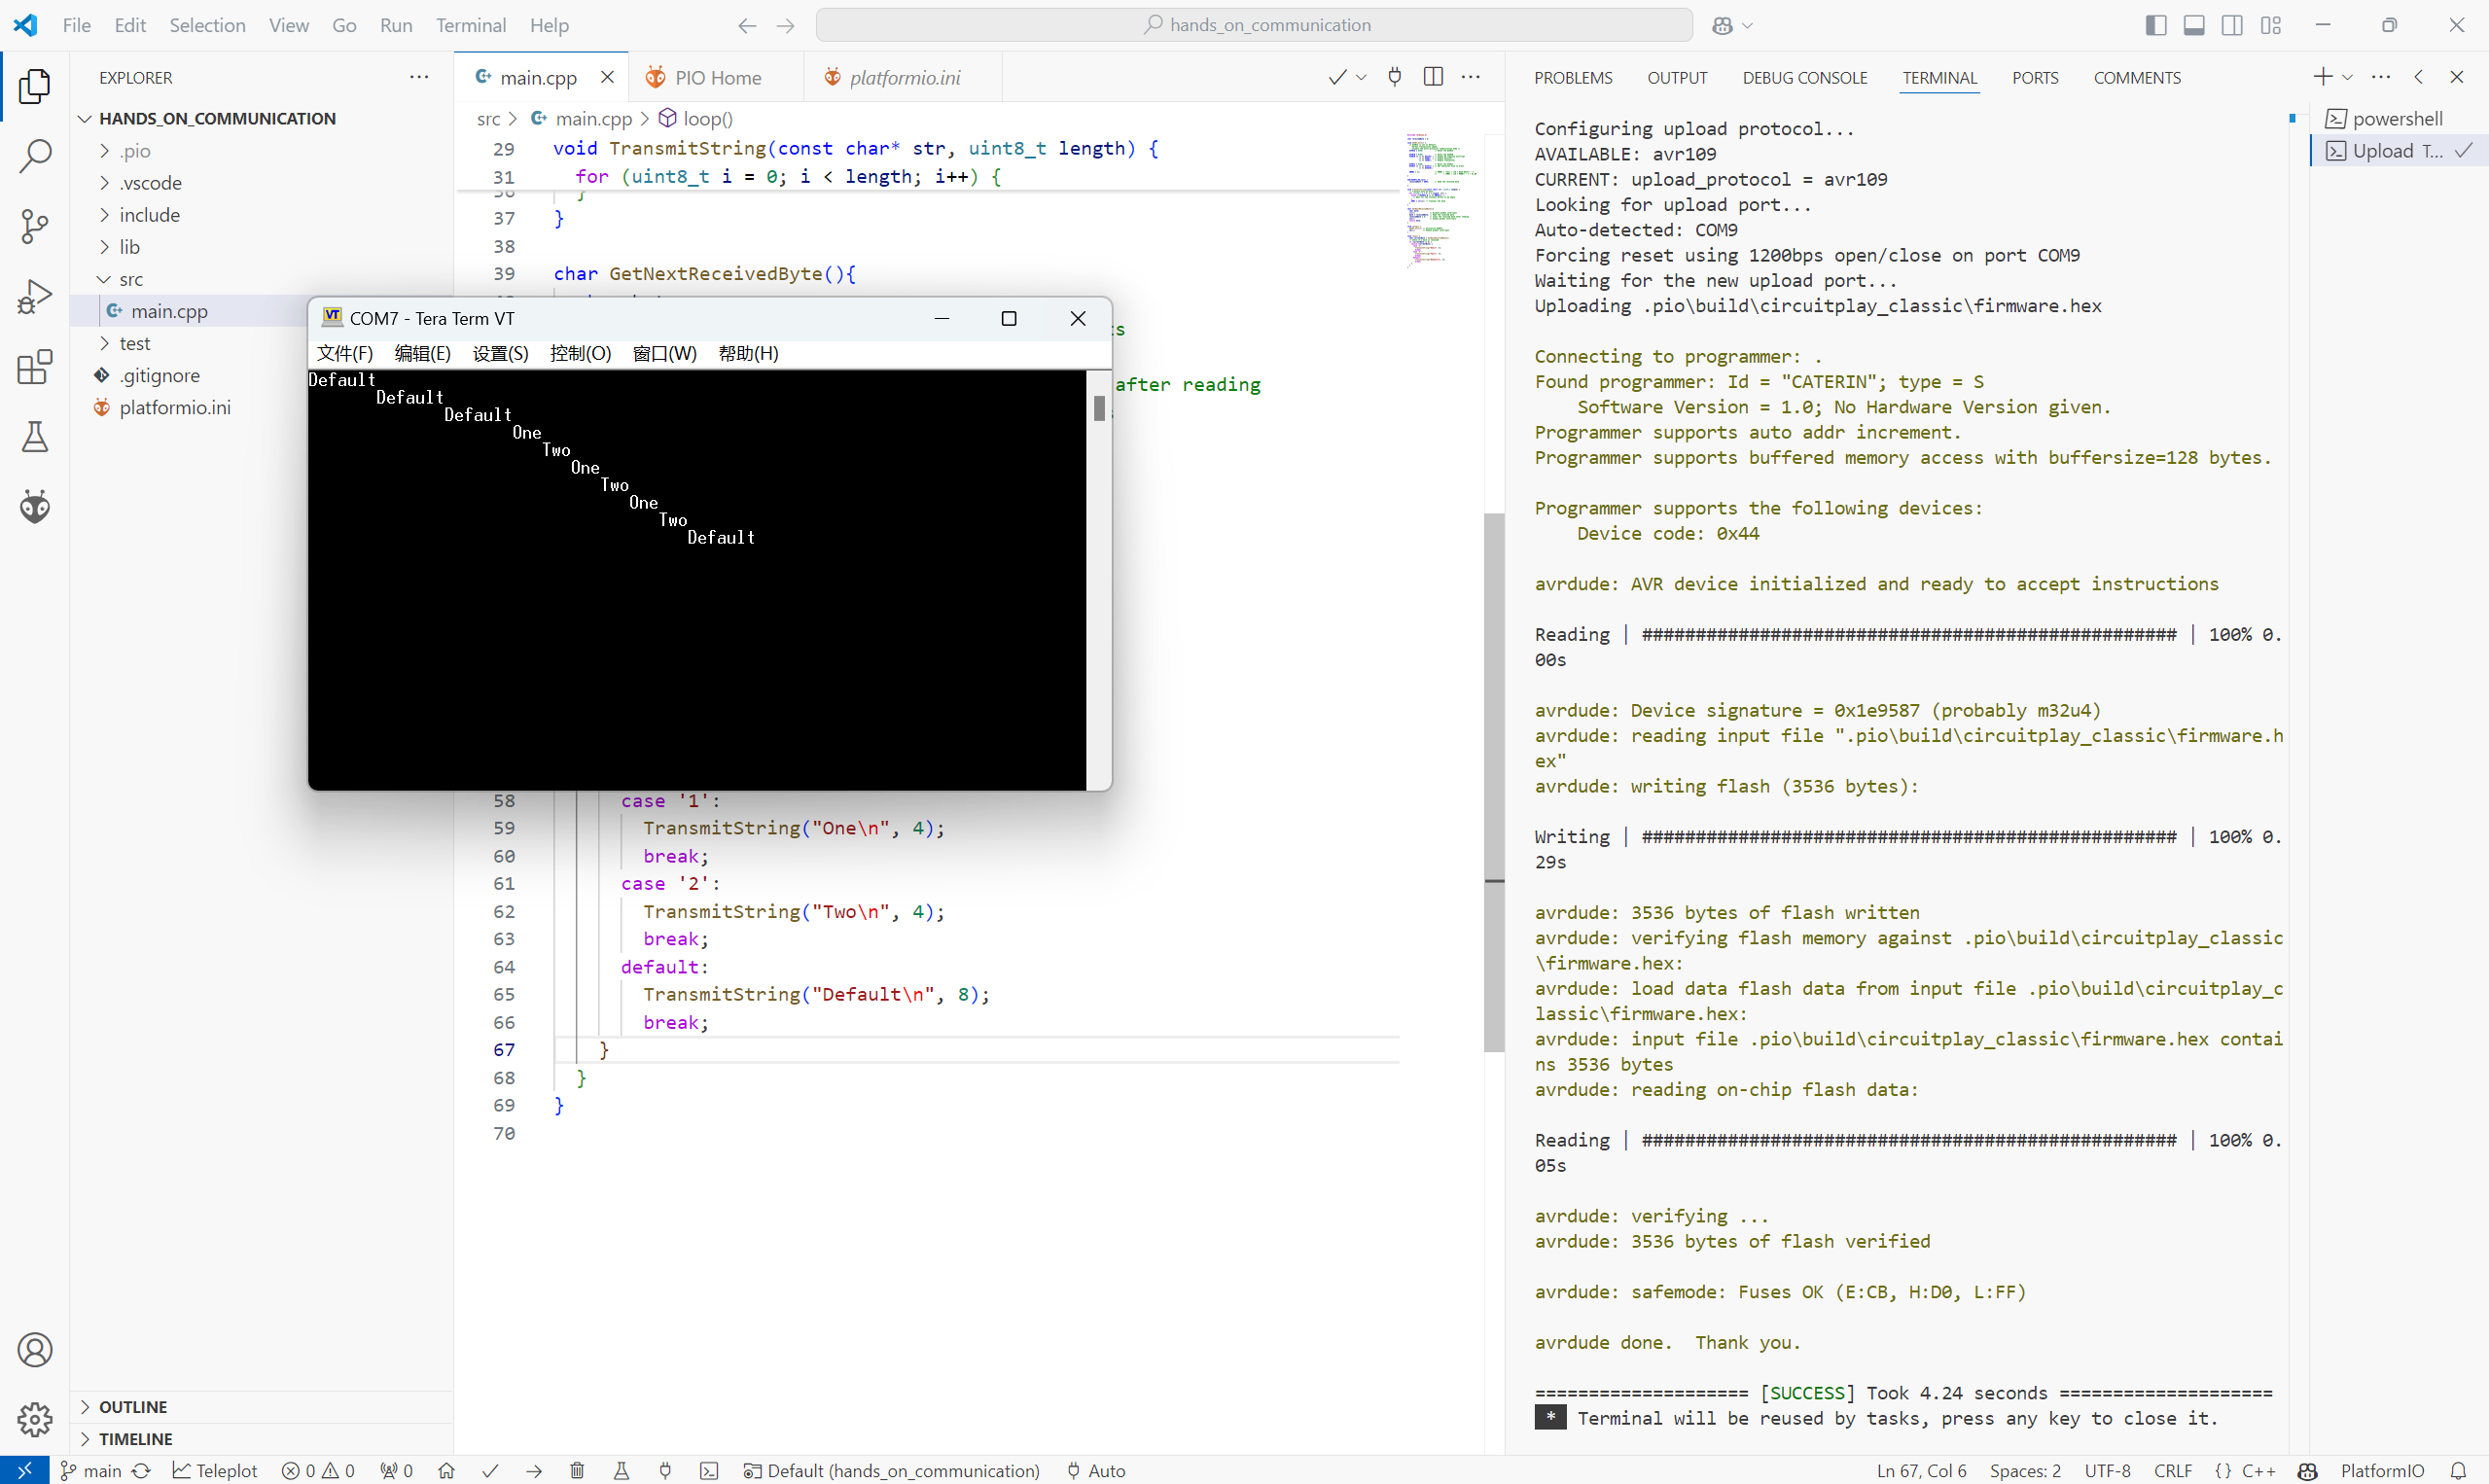
\includegraphics[width=0.8\textwidth]{pic2.png}
    \caption{Output of the program}
\end{figure} \\
which is as expected. 
\end{document}